\chapter{Introduction}

\section{Contexte}


\section{Formulation du problème de propagation d'interface}

\subsection{Formulation lagrangienne traditionnelle}

\subsection{Principe de Huygens avec condition d'entropie}


\section{Cadre de la thèse}


\section{Représentation par les frontières}




\begin{figure}
	\centering
	\colorlet{topo_color}{mycolor_5}
\colorlet{orient_color}{topo_color!60!mycolor_2}
\colorlet{group_color}{topo_color!40!mycolor_3}
\colorlet{geom_color}{mycolor_1}%{mycolor_3}
\def\bigsep{5mm}
\def\smallsep{2.5mm}
\pgfdeclarelayer{bg}    % declare background layer
\pgfsetlayers{bg,main}  % set the order of the layers (main is the standard layer)
\begin{tikzpicture}[
	x = 30mm,
	y = 9.75mm,
	arrow/.style={thick, -stealth', shorten <= 2pt, shorten >= 2pt},
	bounded/.style={arrow, dash pattern=on 4pt off 2pt},
	described/.style={arrow},
	composed/.style={arrow, dash pattern=on 1.5pt off 1.5pt},
	box/.style={rectangle, rounded corners=0.8ex},
	number/.style={font=\footnotesize},
	topo/.style={fill=topo_color!33!white},
	geom/.style={fill=geom_color!33!white},
	orient/.style={fill=orient_color!33!white},
	group/.style={fill=group_color!33!white},
	type/.style={font=\bfseries},%, anchor=east},
	label/.style={anchor=west, inner sep=2pt, font=\scriptsize},
	class/.style={dotted, thick, line cap=round},
	bigclass/.style={class, rounded corners=\bigsep, dash pattern=on 0.8pt off 3.2pt},
	smallclass/.style={class, rounded corners=\smallsep, dash pattern=on 0.3pt off 2.8pt},
	]
	% entités topologiques
	\node[box, topo] at (-1,1) (volume) {Solide};
	\node[box, topo] at (0,1) (face) {Face};
	\node[box, topo] at (1,1) (edge) {Arête};
	\node[box, topo] at (2,1) (vertex) {Sommet};
	% entités de groupement
	\node[box, group] at (-1,3) (shell) {Coquille};
	\node[box, group] at (0,3) (wire) {Contour};
	% entités d'orientation
	\node[box, orient] at (1,3) (halfedge) {Co-arête};
	% entités géométriques
	\node[box, geom] at (0,-1) (surface) {Surface};
	\node[box, geom] at (1,-1) (curve) {Courbe};
	\node[box, geom] at (2,-1) (point) {Point};
	%
	% relations "décrit par"
	\draw[described] (face) -- (surface);
	\draw[described] (edge) -- (curve);
	\draw[described] (vertex) -- (point);
	% relations "délimité par"
	\draw[bounded] (volume) -- 
		node[number,left]{$1+n_{\mathrm{s}}^{\mathrm{int}}$} 
		(shell);
	\draw[bounded] (face) -- 
		node[number,right]{$1+n_{\mathrm{w}}^{\mathrm{int}}$} 
		(wire);
	\draw[bounded] (edge) -- node[number,above]{$2$} (vertex);
	% relations "composé de"
	\draw[composed] (shell) -- node[number,above right]{$n$} (face);
	\draw[composed] (wire) -- node[number,above]{$n$} (halfedge);
	\draw[composed] (edge) -- node[number,right]{$2$} (halfedge);
	%
	% noms de classes
	\gettikzxy{(current bounding box.east)}{\xbbE}{\ybbE}%
	\node[type, geom_color!90!gray] (geomet) at (-1,-1) {Géométrie};
	\node[type, anchor=east, orient_color!90!gray] (orientation) at ({\xbbE-0.5*\smallsep},3) {Orientation};
	\gettikzxy{(halfedge.east)}{\xhE}{\yhE}%
	\gettikzxy{(orientation.west)}{\xoW}{\yoW}%
	\gettikzxy{(shell.west)}{\xsW}{\ysW}%
	\node[type, anchor=east, group_color!90!gray] (grouping) at ({\xsW-\xoW+\xhE},3) {Groupement};
	\gettikzxy{(grouping.west)}{\xgrW}{\ygrW}%
	\gettikzxy{(grouping.south)}{\xgrS}{\ygrS}%
	\gettikzxy{(volume.south)}{\xvS}{\yvS}%
	\node[type, anchor=west, topo_color!90!gray] (topology) at (\xgrW,{0.5*(\ygrS-\smallsep + \yvS-\bigsep)}) {Topologie};
	%
	% classes
	\gettikzxy{(vertex.south east)}{\xtSE}{\ytSE}%
	\gettikzxy{(shell.north)}{\xtN}{\ytN}%
	\gettikzxy{(grouping.west)}{\xtW}{\ytW}%
	\gettikzxy{(geomet.west)}{\xgeW}{\ygeW}%
	\gettikzxy{(topology.north)}{\xtM}{\tmp}%
	\gettikzxy{(grouping.south)}{\tmp}{\ytM}%
	\gettikzxy{(halfedge.south west)}{\xoSW}{\yoSW}%
	\gettikzxy{(halfedge.north)}{\xoN}{\yoN}%
	\gettikzxy{(orientation.north east)}{\xoNE}{\yoNE}%
	\gettikzxy{(grouping.south west)}{\xgrSW}{\ygrSW}%
	\gettikzxy{(wire.south)}{\xgrS}{\ygrS}%
	\gettikzxy{(wire.north east)}{\xgrNE}{\ygrNE}%
	\gettikzxy{(surface.south)}{\xgeS}{\ygeS}%
	\gettikzxy{(surface.north)}{\xgeN}{\ygeN}%
	\begin{pgfonlayer}{bg}    % select the background layer
		\draw[bigclass, topo_color, fill=topo_color!8!white] 
		({\xtSE+\bigsep},{\ytSE-\bigsep}) --
		({\xtSE+\bigsep},{\ytN+\bigsep}) --
		({\xtW-\bigsep},{\ytN+\bigsep}) --
		({\xtW-\bigsep},{\ytSE-\bigsep}) -- cycle;
		%
		\draw[smallclass, orient_color, fill=orient_color!8!white] 
		({\xoSW-\smallsep},{\yoSW-\smallsep}) -- 
		({\xoNE+\smallsep},{\yoSW-\smallsep}) -- 
		({\xoNE+\smallsep},{\yoN+\smallsep}) -- 
		({\xoSW -\smallsep},{\yoN+\smallsep}) -- cycle;
		%
		\draw[smallclass, group_color, fill=group_color!8!white] 
		({\xgrSW-\smallsep},{\ygrS-\smallsep}) -- 
		({\xgrNE+\smallsep},{\ygrS-\smallsep}) -- 
		({\xgrNE+\smallsep},{\ygrNE+\smallsep}) -- 
		({\xgrSW -\smallsep},{\ygrNE+\smallsep}) -- cycle;
		%
		\draw[bigclass, geom_color, fill=geom_color!8!white]
		({\xgeW-\bigsep},{\ygeS-\bigsep}) -- 
		({\xtSE+\bigsep},{\ygeS-\bigsep}) -- 
		({\xtSE+\bigsep},{\ygeN+\bigsep}) -- 
		({\xgeW-\bigsep},{\ygeN+\bigsep}) -- cycle;
	\end{pgfonlayer}
	% légende des relations
	\coordinate (lgd) at ({\xtW-\bigsep+2pt},{0.5*(\ygeS+\ygeN)});
	\foreach \i in {0,1,2}{
		\coordinate (L\i) at ([yshift={-(\i-1)*2.8ex}]lgd);
		\coordinate (R\i) at ([xshift=7.5mm]L\i);
	}
	\draw[described] (L0) -- (R0) node[label] (lbl0) {décrit par};
	\draw[bounded]   (L1) -- (R1) node[label] (lbl1) {délimité par};
	\draw[composed]  (L2) -- (R2) node[label] (lbl2) {composé de};
	\node[draw=black!25,
	inner sep=2pt,
	rounded corners=\smallsep,
	fit={(L0) (lbl0) (lbl1) (lbl2)}] {};
\end{tikzpicture}
	\caption{Hiérarchie des éléments constituant un modèle \brep.}
	\label{fig:BRep_hierarchy}
\end{figure}

\begin{figure}
	\centering
	\setlength{\imagewidth}{80mm}%
\setlength{\imageheight}{\imagewidth}%
\DTLsetseparator{,}%
\DTLloaddb[noheader,keys={x,y,a}]{dbverts}{figures/data/BRep/verts_xya.dat}%
\begin{tikzpicture}[%
	x=\imagewidth, y=\imageheight,
	img/.style={anchor=south west, inner sep=0}]
	%%%%%%%%%%%%%%%% SHELL %%%%%%%%%%%%%%%%
	%%% FACES
	\node[img] at (0,0) {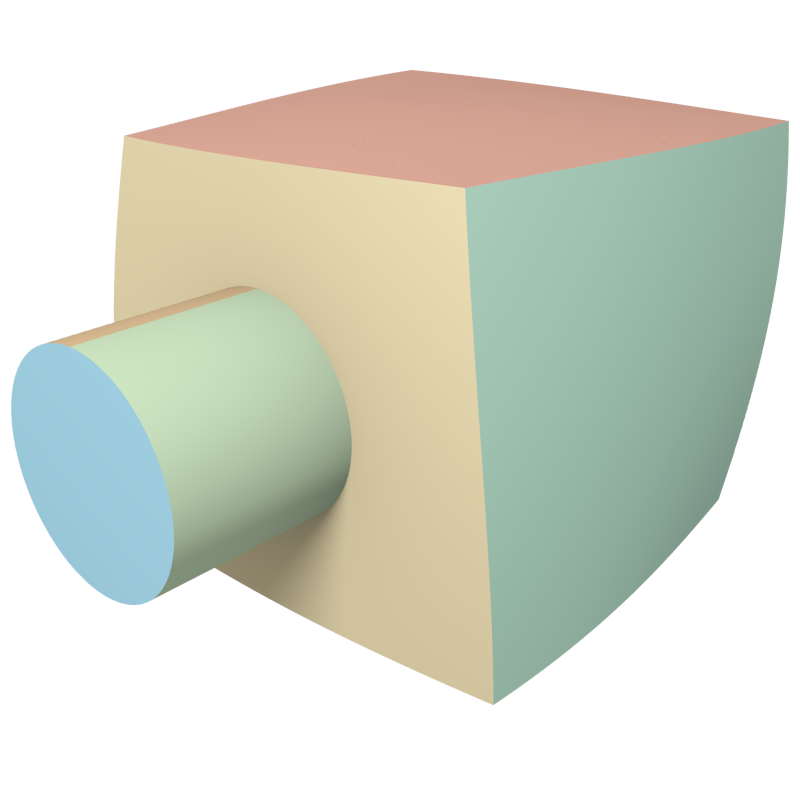
\includegraphics[width=\imagewidth]{BRep/shell}};
	%%% HIDDEN EDGES
	\node[img] at (0,0) {
\includegraphics[width=\imagewidth]{BRep/edges_hidden}};
	%%% HIDDEN VERTICES
	\DTLforeach*{dbverts}{\locx=x, \locy=y, \loca=a}{%
		\ifnum \loca = 0
			\fill[black] (\locx,\locy) circle (1.0pt);
		\fi
	}%
	%%% FACES (semi-transparent to mask hidden edges & verts)
	{\transparent{0.75}
		\node[img] at (0,0) {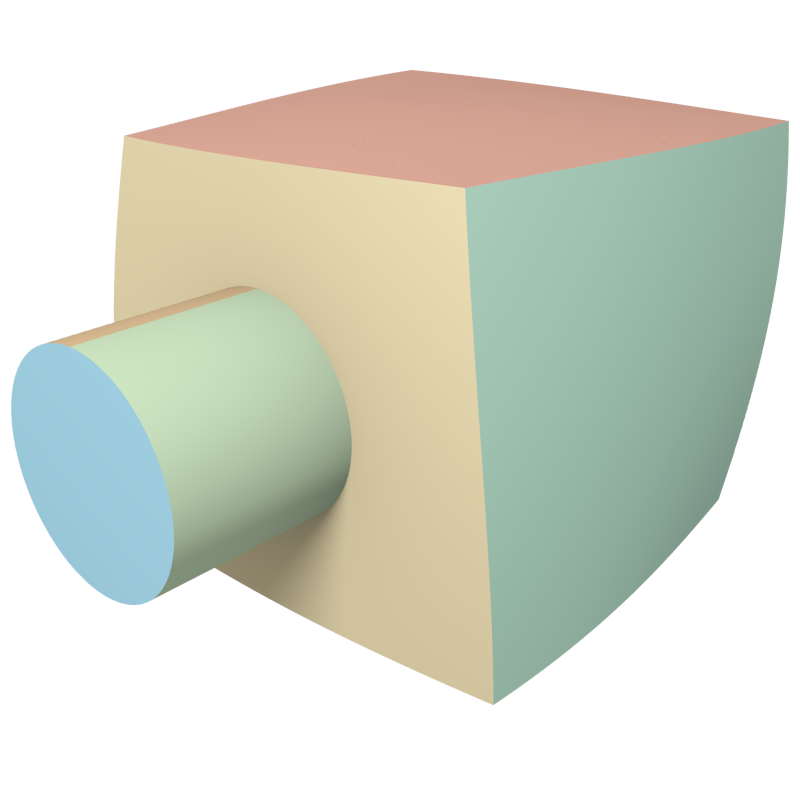
\includegraphics[width=\imagewidth]{BRep/shell}};
	}%
	%%% VISIBLE EDGES
	\node[img] at (0,0) {
\includegraphics[width=\imagewidth]{BRep/edges_visible}};
	%%% VISIBLE VERTICES
	\DTLforeach*{dbverts}{\locx=x, \locy=y, \loca=a}{%
		\ifnum \loca = 1
			\fill[black] (\locx,\locy) circle (1.0pt);
		\fi
	}%
\end{tikzpicture}
\DTLgdeletedb{dbverts}%
%%%%%%%%%%%%%%%%%%%%%%%%%%%%%%%%%%%%%%
%
%%%%%%%%%%%%%%%% FACES %%%%%%%%%%%%%%%%
\def\imfacew{44mm}
\def\ngriduv{6}
\def\vertsep{0.05}
\def\edglabsepuv{0.17}
\def\wirlabsepuv{0.18}
\def\edglabsepxyz{0.06}
\def\iniwclr{0.3}
\def\decwclr{0.3}%{0.2}
\def\uvscale{0.34}
\def\uvyshift{-0.7}
\pgfmathsetmacro\sepyshift{0.5 * (\uvyshift+\uvscale)}%
%
\begin{tikzpicture}[%
	x = \imfacew, y = \imfacew,
	gridtick/.style={red, fill=white, font=\tiny, inner sep=0.5pt},
	img/.style={anchor=south west, inner sep=0},
	label/.style={inner sep=1pt, font=\scriptsize},
	uvgrid/.style={black!10!white},
	curv/.style={line width=0.8pt, line cap=round},
	spacelabel/.style={anchor=north, rotate=90, inner sep=0, font=\bfseries},
	]
	\foreach \jfa/\ifa in {-1/007, 0/008, 1/002}{%
		\figbrepface{\ifa}{{1.05*\jfa - 0.5}}{{-\sepyshift}}%\hfill
	}%
	\draw[very thick, gray, dashed] 
	({-0.5*\textwidth},0) -- ++ 
	(\textwidth,0);
	\node[spacelabel] (xyzspace) at 
	({-0.5*\textwidth},{-\sepyshift+0.5}) {Espace euclidien\vphantom{Espace paramétrique}};
	\node[spacelabel] (uvspace) at 
	({-0.5*\textwidth},{\sepyshift-\uvscale}) {Espace paramétrique\vphantom{Espace euclidien}};
\end{tikzpicture}

	\caption{Modèle \brep.}
	\label{fig:BRep}
\end{figure}

\begin{figure}
	\centering
	\setlength{\imagewidth}{67.5mm}
\setlength{\imageheight}{\imagewidth * \real{0.75}}
%
\def\uvscale{0.28}
\def\fracaxeoffset{0.0}
\def\distanceaxe{0.1}
\def\psisep{-0.42}
%
\DTLsetseparator{,}%
\DTLloaddb[noheader,keys={x,y}]{dbpoint}{figures/data/simple_intersection/point.dat}%
\DTLassign{dbpoint}{1}{\xloc=x, \yloc=y}% 
%
\begin{tikzpicture}[
	x=\imagewidth, y=\imageheight, 
	axe/.style={-stealth, line width=0.5pt},
	uvdomain/.style={thin}, 
	image/.style={anchor=south west, inner sep=0},
	curve/.style={thick, line cap=round},
	label/.style={font=\normalsize},
	axelabel/.style={font=\small},
	axeuvlabel/.style={axelabel, inner sep=0},
	point/.style={fill=black, circle, scale=0.3},
	map/.style={-{Classical TikZ Rightarrow[length=4pt,width=4pt]}}]
	%
	\node[image] (img) at (0,0) {
\includegraphics[width=\imagewidth]{figures/images/simple_intersection/surfaces}};
	\node[image] (img) at (0,0) {
\includegraphics[width=\imagewidth]{figures/images/simple_intersection/borders_hidden}};
	{\transparent{0.75}%
		\node[image] (img) at (0,0) {
\includegraphics[width=\imagewidth]{figures/images/simple_intersection/surfaces}};
	}%
	\node[image] (img) at (0,0) {
\includegraphics[width=\imagewidth]{figures/images/simple_intersection/borders_visible}};
	\draw[curve] plot file {figures/data/simple_intersection/curve_xy.dat};
	\node[point] (xyz) at (\xloc, \yloc) {};
	\node[label, anchor=east] at (\xloc, \yloc) {$\bg(w)$};
	%
	\node[label] at (0.56, 0.91) {$\Sigma_1$};
	\node[label] at (0.93, 0.75) {$\Sigma_2$};
	%
%	\foreach \igrid in  {0,0.1,...,1.01}{
%		\draw[red, thin] (0,\igrid) -- (1,\igrid)
%		                 (\igrid,0) -- (\igrid,1);
%	}
	% 
	% trièdre
	\def\scaletriedre{0.8}
	\coordinate (o) at (0.13209545612335205 , 0.14773482084274292);
	\coordinate (x) at (0.23464959859848022 , 0.02938912808895111);
	\coordinate (y) at (0.26169726252555847 , 0.2535654902458191);
	\coordinate (z) at (0.1061694324016571 , 0.31903284788131714);
	\draw[axe] (o) -- ($(o)!\scaletriedre!(x)$) node[axelabel, anchor=west] {$x$};
	\draw[axe] (o) -- ($(o)!\scaletriedre!(y)$) node[axelabel, anchor=west] {$y$};
	\draw[axe] (o) -- ($(o)!\scaletriedre!(z)$) node[axelabel, anchor=south] {$z$};
	%
	\begin{scope}[scale=\uvscale, x=\imageheight, y=\imageheight, shift={(img.west)}]
		\begin{scope}[shift={(-1.5,0.7)}]
			\DTLloaddb[noheader,keys={r,g,b}]{dbsurfacecolor}{figures/data/BRep/faces/facecolor_002.dat}%
			\DTLassign{dbsurfacecolor}{1}{\rfai=r,\gfai=g,\bfai=b}% 
			\definecolor{surfacecolor}{RGB}{\rfai,\gfai,\bfai}
			\draw[uvdomain, fill=surfacecolor] (-1,-1) -- (1,-1) -- (1,1) -- (-1,1) -- cycle;
			\DTLgdeletedb{dbsurfacecolor}
			%
			\draw[curve] plot file {/d/bandrieu/GitHub/FFTsurf/test/demo_intersection/simple/curve_uv1.dat};
			%
			\DTLassign{dbpoint}{2}{\uloc=x, \vloc=y}% 
			\DTLassign{dbpoint}{3}{\duloc=x, \dvloc=y}% 
			\node[point] (uv1) at (\uloc, \vloc) {};
			%\node[label] at ({\uloc + \psisep*\duloc}, {\vloc + \psisep*\dvloc}) {$\bp_1(w)$};
			\node[label, anchor=north east, inner sep=0] at (\uloc, \vloc) {$\bp_1(w)$};
			% Axes
			\coordinate (o) at ({-1-\distanceaxe},{-1-\distanceaxe});
			\draw[axe] (o) -- ++ ({\fracaxeoffset+\distanceaxe+0.5},0) node [axeuvlabel, anchor=north west] {$u_1$};
			\draw[axe] (o) -- ++ (0,{\fracaxeoffset+\distanceaxe+0.5}) node [axeuvlabel, anchor=south east] {$v_1$};
		\end{scope}
	\end{scope}
	%
	\begin{scope}[scale=\uvscale, x=\imageheight, y=\imageheight, shift={(img.east)}]
		\begin{scope}[shift={(1.6,-0.9)}]
			\DTLloaddb[noheader,keys={r,g,b}]{dbsurfacecolor}{figures/data/BRep/faces/facecolor_008.dat}%
			\DTLassign{dbsurfacecolor}{1}{\rfai=r,\gfai=g,\bfai=b}% 
			\definecolor{surfacecolor}{RGB}{\rfai,\gfai,\bfai}
			\draw[uvdomain, fill=surfacecolor] (-1,-1) -- (1,-1) -- (1,1) -- (-1,1) -- cycle;
			\DTLgdeletedb{dbsurfacecolor}
			%
			\draw[curve] plot file {/d/bandrieu/GitHub/FFTsurf/test/demo_intersection/simple/curve_uv2.dat};
			%
			\DTLassign{dbpoint}{4}{\uloc=x, \vloc=y}% 
			\DTLassign{dbpoint}{5}{\duloc=x, \dvloc=y}% 
			\node[point] (uv2) at (\uloc, \vloc) {};
			%\node[label] at ({\uloc + \psisep*\duloc}, {\vloc + \psisep*\dvloc}) {$\bp_2(w)$};
			\node[label, anchor=north east, inner sep=0] at (\uloc, \vloc) {$\bp_2(w)$};
			% Axes
			\coordinate (o) at ({-1-\distanceaxe},{-1-\distanceaxe});
			\draw[axe] (o) -- ++ ({\fracaxeoffset+\distanceaxe+0.5},0) node [axeuvlabel, anchor=north west] {$u_2$};
			\draw[axe] (o) -- ++ (0,{\fracaxeoffset+\distanceaxe+0.5}) node [axeuvlabel, anchor=south east] {$v_2$};
		\end{scope}
	\end{scope}
	%
	% mappings
	\draw [map, shorten <= 5mm, shorten >= 5mm] (uv1) to [bend left =40] node [label, anchor=south west] {$\bs_1$} (xyz);
	\draw [map, shorten <= 5mm, shorten >= 5mm] (uv2) to [bend right=40] node [label, anchor=south west] {$\bs_2$} (xyz);
	%
%	\draw[red, thin, dashed] (current bounding box.south west) rectangle (current bounding box.north east);
\end{tikzpicture}
\DTLgdeletedb{dbpoint}
	\caption{Description géométrique d'une arête \brep.}
\end{figure}




\section{Contributions}



\begin{enumerate}
	\item mise en place d'un \anglais{framework} pour résoudre la propagation d'une interface 3d \textbf{régulière par morceaux} représentée par un modèle \brep
	\begin{enumerate}
		\item mise au point d'un algorithme basé sur le \textbf{principe de Huygens} (avec condition d'entropie) pour \textbf{adapter dynamiquement la géométrie et la topologie} du modèle \brep\ de l'interface au cours de la propagation (autrement dit, la validité du modèle \brep\ est maintenue tout au long de la propagation)
	\end{enumerate}


	\item utilisation du \textbf{formalisme \brep\ }pour représenter une interface \textbf{régulière par morceaux} en propagation en 3d (dans des applications de type interaction fluide-structure, combustion de solide dans un fluide)
	\item mise au point d'un algorithme basé sur le \textbf{principe de Huygens} (avec condition d'entropie) pour \textbf{adapter dynamiquement la géométrie et la topologie} du modèle \brep\ de l'interface au cours de la propagation
	\item (mise en \oe uvre d'une méthode pseudo-spectrale (\ie d'ordre élevé) (utilisant les polynômes de Chebyshev comme fonctions de base) pour suivre \textbf{efficacement et avec une grande précision} le mouvement de l'interface)
	\item mise en \oe uvre d'une méthodologie pour adapter un \textbf{maillage dynamique géométriquement fidèle au modèle \brep\ dynamique} de l'interface, dans le but de réaliser des simulations EF/VF
\end{enumerate}


\section{Organisation du manuscrit}